
\documentclass[conference]{IEEEtran}
\usepackage{url}
\usepackage{graphicx}

\begin{document}


\title{Patient Consent}

\author{\IEEEauthorblockN{Atif Khan, Sarah Nadi}
\IEEEauthorblockA{David R. Cheriton School of Computer Science\\
University of Waterloo\\
Ontario, Canada\\
{??, snadi}@uwaterloo.ca}
}

% make the title area
\maketitle


\begin{abstract}
The abstract goes here.
\end{abstract}



\section{Introduction}
With the advance of Information Communication Technologies (ICT), more medical organizations are utilizing electronic systems to capture, manage and use patient
related information.  The scope of this information varies from organization wide Electronic Medical Records (EMRs) to Electronic Health Records (EHRs) shared
between different organizations.  Although this improves the effectiveness of information exchange, coordination, and use, it also raises the critical issue of
patient consent. Usually, patient information is collected for the primary purpose of providing health care for a specific episode. Any secondary use must be in
accordance with patient consent.  It has been argued that a patient should be aware of all the systems collecting their information, and should be able to
specify how this information can be used~\cite{kluge2004informed}. Ideally, in an electronic system, the system would automatically grant or deny permission to
accessing a patient's record according to their specific consent policy. However, it is often difficult, if not impossible, to predict all future-use scenarios
and enforce patient consent in an appropriate manner.

There are many aspects of this problem that need to be solved. First, how can patient consent be captured electronically in an effective way? Second, how can
the captured consent policies be represented and processed internally? Finally, how can we define consent policies that protect the patient privacy, but do not
compromise their health at the same time? All three problems are very important in this domain. However, in this paper, we focus on the second problem, and
briefly touch upon the third.


To address these problems, we propose building a policy based patient consent management system. The system would utilize (previously captured) patient consent
information and various operational policies as input. Each policy will be represented by a set of RDF rules in Notation 3 (N3)~\cite{N3not}.  We will use the
Euler proof mechanism~\cite{eurlorprf} to compute (a) the result and (b) the proof of the aggregated rules.  


Our goal is to demonstrate that various actions on patient information can be protected in a real-time manner by utilizing the policy based consent management.
The advantage of using Euler to generate a proof is that in the future, proofs can be validated between different systems when exchanging EHRs. This offers a
major improvement over the current industry practice of patient consent management and secondary use of patient information. This paper describes the
preliminary effort in this direction where we illustrate the applicability of our idea through a selection of consent policies and situations.


The contributions of this work are as follows: 

\begin{itemize}
    \item A set of consent policies represented in N3 notation. These are expressed as N3 rules which allow or deny access to the specified documents.

\item A collection of executable scenarios that show how the consent policies are applied in different situations. A Java application is developed to demonstrate these scenarios.

\item Policy conflict detection (We still need more details about this part)
\end{itemize}

The rest of this paper is organized as follows. Section~\ref{bg-sec} provides background information about patient consent, N3 notation, and the Euler engine. Section~\ref{rel-work} describes some of the work that has been done to develop an electronic patient consent system. Section~\ref{cons-polic} explains the different consent policies, and which ones will we be including in our prototype. Section~\ref{main-sys} describes the prototype system developed in this work. It describes how the information flow in the system as well as the policy rules and facts used. This section also mentions the current limitations of the system. Section~\ref{discFuture} discusses ??, and outlines possible future additions to the system. Finally, Section~\ref{concl} concludes this paper.

\section{Background}
\label{bg-sec}

\subsection{Patient Consent}
\label{pat-consent}
Background of what patient consent is (accessing records vs consent to an operation for example).

Historically, patient consent was through paper (brief summary of how it went)


\subsection{N3 Notation}

Brief summary of N3 notation

\subsection{Euler}

Brief summary of how Euler works and how it provides a proof. Mention things like one query per file, and first match only etc.


\section{Related Work}
\label{rel-work}

Work that addresses patient consent for access of electronic records.


\section{Consent Policies}
\label{cons-polic}

There are different forms of consent that a patient may choose from. Coiera and Clarke~\cite{coiera2004consent} define four general forms of patient consent as
follows:

\begin{itemize}
 \item \textit{General consent}: This is also generally known as ``opt-in'' which means that the patient agrees that any health care professional may access
all of their health data for the purpose of providing care to them.
\item \textit{General consent with specific denial(s)}: This means that the patient specifically defines certain exceptions to their general consent policy.
These exceptions may be related to particular data or to particular people.
\item \textit{General denial with specific consent(s)}: In this case, the patient generally denies access to their data except in specific circumstances. These
may include disclosure for specific purposes or to specific people or the disclosure of certain types of information.
\item \textit{General denial}: This is the strictest level of consent a patient may have. In this case, the patient denies the use of their information for any
future event irrelevant of the circumstances that may occur. This consent policy is also generally known as ``opt-out''.
\end{itemize}

Pruski~\cite{pruski2010} use these four forms of consent while designing their rule-based language for describing patient consent policies. Additionally,
Pruski outlines the key requirements that must be taken into consideration while dealing with patient consent. These are expressing who can access the data,
the kind and the sensitivity of the data, the period for which a consent policy is valid, the purpose of why the data is being accessed, and what kind of
consent is given to the user requesting the data. 

In our work, we consider both the four forms of patient consent as well as some of the requirements proposed by Pruski. In our current prototype, we support
five types of patient consent policies as follows:

\begin{itemize}
 \item \textit{opt-in}: As described above, a patient who has an opt-in policy allows any treating doctor to access their information. In our system, we also
add other conditions that need to be met such as that the health care professional should be a member of the admitting organization etc. These details will be
discussed in Section~\ref{main-sys}.
\item \textit{opt-in except for sensitive documents}: In this case, the patient allows access to all their information except for documents that are classified
as sensitive. For example, these may include HIV tests or Sexually Transmitted Diseases. 
\item \textit{opt-in except for certain people}: In this case, the patient allows access to all their information, but specifically denies certain individuals
from accessing their data.
\item \textit{opt-out}: A patient with an opt-out policy explicitly denies access to all their information regardless of who is trying to access the data or
why they are trying to access it.
\item \textit{opt-out with emergency override}: In this case, the patient agrees to grant access to their information only if it is an emergency situation. 
\end{itemize}

\section{Our System Name}
\label{main-sys}

Not sure of this section's title but if we have a name for our system, that would do for the title. 

\subsection{Information Flow}
\label{info-flow}

Currently, our system assumes that all the information needed is already captured. That is, all information about the patient, their documents as well as their
privacy policies. Similarly, we also assume that all the information about the different hospitals, doctors, and nurses is already present. In this sense, we
focus on answering the question of whether a doctor or nurse can access a certain document. This is done by loading the facts available and our rule set into
Euler, and then querying it to see if a certain doctor or nurse can access a certain document. If access is granted, then we present the user with the proof
provided by Euler. If no proof is found, we check if we can find an explicit deny rule for the same actors in the original query. If so, we present the user
with the proof of why access has been denied.

PUT SNAPSHOTS HERE

\subsection{Access Policies in N3 Notation}
\label{rules-sec}

Describes our rules/policy file. 

\subsection{Facts in N3 Notation}

\begin{figure*}[t]
\centering
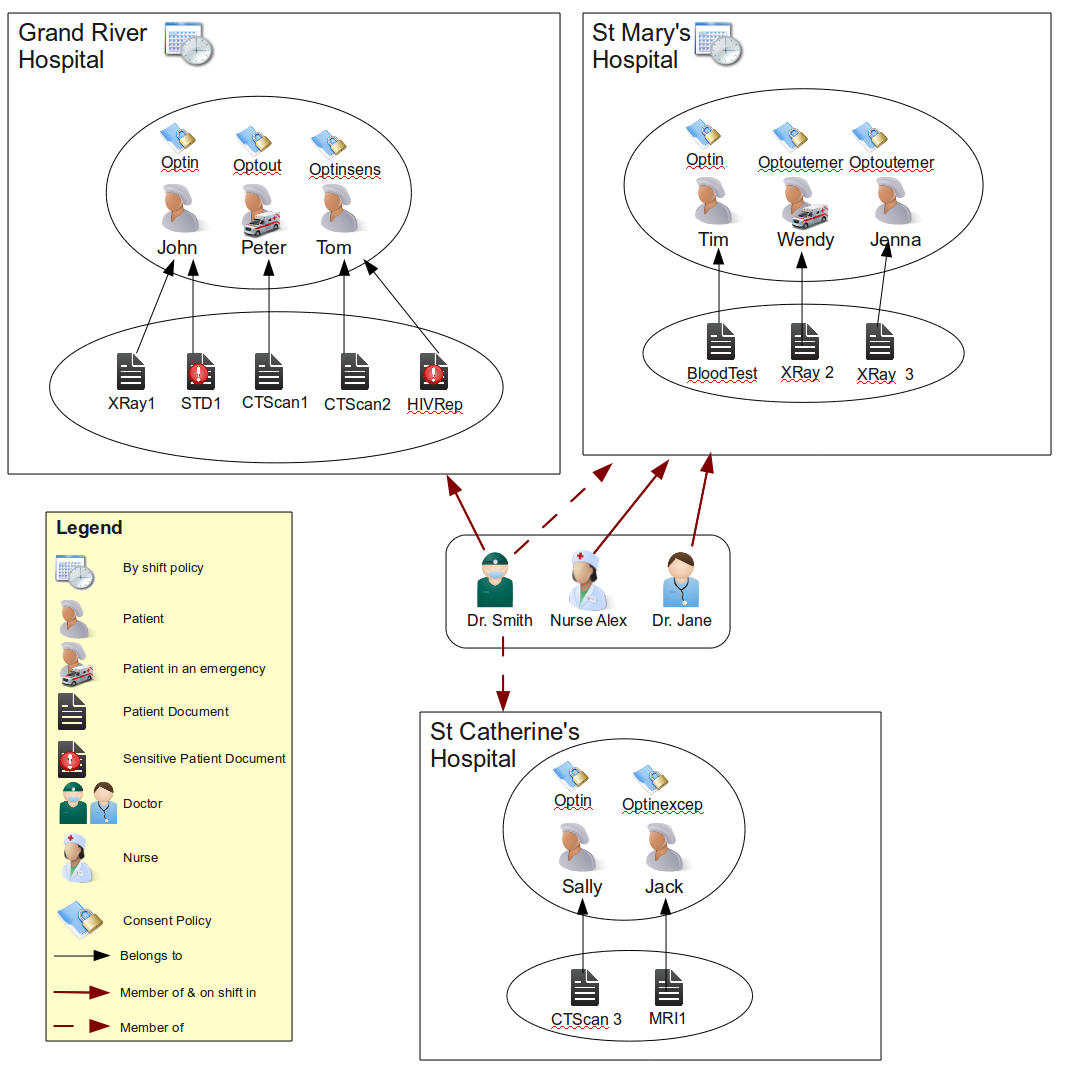
\includegraphics[width=16cm,height=14cm]{BigPicture.png}
\caption{test}
\label{fig:allfacts}
\end{figure*}


Describes the facts we support (different entities and relationships) in our facts file.

\subsection{Limitations}

Describes the current limitations of our system

\section{Discussion and Future Work}
\label{discFuture}

can split into two sections if there's a lot of things to discuss


\section{Conclusion}
\label{concl}
The conclusion goes here.




% conference papers do not normally have an appendix


% use section* for acknowledgement
\section*{Acknowledgment}


The authors would like to thank Dr. Helen Chen for ...





%\IEEEtriggeratref{8}
% references section
\bibliographystyle{IEEEtran}
\bibliography{references}




% that's all folks
\end{document}


